\documentclass[a4paper,11pt,final]{article}


\usepackage{listings}

% Include all necessary packages

\usepackage{listings}								% For code segments
\usepackage{color}									% For text, links and code highlighting
\usepackage[pdftex]{hyperref}						% For external and internal links
\usepackage{graphicx}								% For including figures
\usepackage[utf8]{inputenc}							% The package translates various standard and other input encodings into a ‘LaTeX internal language’
\usepackage[T1]{fontenc}							% The package allows the user to select font encodings, and for each encoding provides an interface to ‘font-encoding-specific’ commands for each font.
\usepackage{sectsty}								% A LaTeX2e package to help change the style of any or all of LaTeX's sectional headers in the article, book, or report classes. 
\usepackage[french]{babel}							% The package manages culturally-determined typographical (and other) rules, and hyphenation patterns for a wide range of languages.
\usepackage{geometry}								% The package provides an easy and flexible user interface to customize page layout   
\usepackage{textcomp}								% Supports the Text Companion fonts which provide many text symbols (such as baht, bullet, copyright, musicalnote, onequarter, section, and yen) in the TS1 encoding. 
\usepackage[toc, acronym,style=altlist]{glossaries}	% For build glossary and include an internal link into the table of content. 
\usepackage{index}									% For index.
\usepackage{caption}								% For caption customization

\usepackage{setspace}
\usepackage{hyperref}
%\usepackage[french]{varioref}
\usepackage{setspace}
\usepackage[french]{babel}
\usepackage{fancyhdr}
\usepackage{lastpage}
\usepackage{fancybox}
\usepackage{float}
\usepackage{verbatimbox}


%\usepackage[final]{pdfpages}						% This package simplifies the insertion of external multi-page PDF or PS doc-uments. It supports pdfTeX, VTeX, and XeTeX.
\usepackage{float}									% Improves the interface for defining floating objects such as figures and tables.

\usepackage{amsmath}								% It adapts for use in LaTeX most of the mathematical features found in AMS-TeX
\usepackage{amssymb}								% This file defines all the symbols found in the AMS symbol fonts msam and msbm.
%\usepackage{mathrsfs}

\usepackage{array,longtable}						% Longtable allows you to write tables that continue to the next page
%\usepackage{rotating}								% A package built on the standard LaTeX graphics package to perform all the different sorts of rotation.

\usepackage{amstext}
\usepackage{latexsym}
\usepackage{epsf} 
\usepackage{amsfonts}
\usepackage{sansmath}

\usepackage{stmaryrd}


% Personal command
\newcommand{\MG}{\mathcal{G}}
\newcommand{\ML}{\mathcal{L}}
\newcommand{\MN}{\mathcal{N}}
\newcommand{\MU}{\mathcal{U}}
\newcommand{\MQ}{\mathcal{Q}}
\newcommand{\e}{\mathrm e}
\newcommand{\ind}{\mathbf{1}}
\newcommand{\EMMTETA}{\tilde \theta_{n}}
\newcommand{\XNB}{\bar{X}_{n}}
\newcommand{\dx}{\,dx}
\newcommand{\dt}{\,dt}
\newcommand{\R}{\mathbb{R}}
\newcommand{\N}{\mathbb{N}}
\newcommand{\abs}[1]{\left\lvert#1\right\rvert}
\newcommand{\norm}[1]{\left\lVert#1\right\rVert}


% Personal color definitions

\definecolor{P_GREEN}		{rgb}	{0.0,0.45,0.0}	% Light green 
\definecolor{P_ORANGE}		{rgb}	{1.00,0.65,0.20}	% Light orange
\definecolor{P_GREY}		{rgb}	{0.45,0.45,0.45}	% Medium grey (Eolas grey)
\definecolor{P_BROWN}		{rgb}	{0.40,0.0,0.0}
\definecolor{P_BLUE_DARK}		{rgb}	{0.00, 0.00, 0.205}	% Medium blue (Eolas blue)
\definecolor{P_BLUE}		{rgb}	{0.0, 0.0, 0.40}
%\definecolor{P_BLUE_LIGHT}		{rgb}	{0.33, 0.5, 0.93}
\definecolor{P_BLUE_LIGHT}		{rgb}	{0.0, 0.0, 0.63}
\definecolor{P_RED}			{rgb}	{0.63,0.13,0.13} 	% Dark red (scarlet red)

% Style & color settings

% Style & color for input name in the glossary (blod & light green)
\renewcommand{\glsnamefont}[1]{\color{P_GREEN}{\textbf{#1}}}

% Color of captions (figures, listing, tables) (medium grey)
\captionsetup {
  font = {
    color = P_GREY
  }
}


% Color for each structure part
%%\titlefont     {\color{P_GREY}}
\partfont	 		{\color{P_GREY}}	% Part are set in medium grey
\chapterfont		{\color{P_GREY}}	% Chapter are set in medium grey
\sectionfont		{\color{P_GREEN}}	% Section are set in light green
\subsectionfont		{\color{P_BLUE}}	% Subsection are set in light orange
\subsubsectionfont	{\color{P_BLUE_LIGHT}}	% Subsubsection are set in medium grey



% Table of Content customization

%%
% 	Each sectiontype (chapter, section, ...) has a number associated with it. Two other counters determine when section numbers are printed (secnumdepth) and what sections appear in the table of contents (tocdepth). 
%	Part			=	-1
%	Chapter			=	0
%	Section 		= 	1
%	Subsection		=	2
%	Subsubsection	=	3
%	Paragraph		=	4
%	Subparagraph	=	5
%	
%\setcounter{secnumdepth}{0}	% Chapter are printed
%\setcounter{tocdepth}{4}   	% List parts, chapters, sections, subsections, and subsubsections in the table of contents
%%

% Personnal commands definitions

% Draw an horizontal rule, width of 0.1mm
\newcommand{\HRule} {
  \rule{\linewidth}{0.1mm}
}

% Glossary, index creation

\makeglossaries % Allow glossary creation
\makeindex		% Allow index creation

% Personal link and PDF definitions

\hypersetup{
  pdffitwindow	=	false,     				% Page fit to the window when opened
  %
  pdftitle		=	{Compte rendu},    	% PDF Title (show in reader bar)
  pdfauthor		=	{noname},	% PDF author (show in PDF properties)
  pdfsubject		=	{Test},  				% PDF subject (show in PDF properties)
  pdfkeywords		=	{sample} {example},		% List of keywords (show in the PDF properties)
  pdfcreator		=	{noname},   	% Creator of the PDF (show in the PDF properties)
  pdfproducer		=	{noname},	% Producer of the PDF (show in the PDF properties)
  %
  colorlinks		=	true,       			% False : boxed links; true: colored links
  urlcolor		=	P_BLUE,          		% Color of external links
  linkcolor		=	black,          		% Color of internal links
  citecolor		=	black,        			% Color of links to bibliography
  filecolor		=	black,      			% Color of file links
  %
  pdfnewwindow	=	true      				% Links are displayed / or not in new window
  %
  %bookmarks		=	true,         			% Show / or not bookmarks bar
  %unicode		=	false,          		% Non-Latin characters in Acrobat’s bookmarks
  %pdftoolbar		=	true,        			% Show / or not Acrobat’s toolbar
  %pdfmenubar		=	true,        			% Show / or not Acrobat’s menu
  %pdfstartview	=	{FitH},    				% Fits the width of the page to the window
  %
}

% Personal listing / code definitions

% General settings for listings
\lstset{ %
  %language			=, 														% Set the language of the code
  %
  title				=	\lstname, 											% Show the filename of files included with \lstinputlisting
  caption				=	\lstname,
  %
  frame				=	single, 											% Set / or not the frame style around the code
  backgroundcolor		=	\color{white}, 										% Background color
  %
  basicstyle			=	\footnotesize, 										% Set the size of the font that are used for the code
  %
  breaklines			=	true,												% Allow automatic breakline instead of overflow the listing size limits
  breakindent			=	10pt,												% Indent between code and break character
  breakatwhitespace	=	true,												% Break only on space (not during a word)
  breakautoindent		=	true,                         						% Auto indent after breaking
  prebreak			=	\raisebox{0ex}[0ex][0ex]{\ensuremath{\backslash}},	% Set the character before breaking (ex: int main \)
  %
  %numbers			=	left, 												% Where to put the line-numbers
  %numberstyle		=	\footnotesize, 										% Set the site of the font that are used for lines numbering
  %stepnumber			=	1, 													% Step between two line-number
  %numbersep			=	5pt,												% Indentation between line-numbers and code
  %numberblanklines	=	true,												% Numbering or not blank lines
  %
  showspaces			=	false, 												% Replace / or not spaces by particular underscores
  %showstringspaces	=	false, 												% Underline spaces within strings
  %showtabs			=	false, 												% Replace / or not tabs by particular underscores
  tabsize				=	4, 													% Sets default tabsize to 2 spaces
  %
  captionpos			=	b 													% Set the caption position (b = bottom, t = top, ...)
  %
}

% Add the CLI as a language for listing
\lstdefinelanguage{cli} {
  morekeywords={install},		
  otherkeywords={apt-get},
  morecomment=[l]\#,			% Each begining with the '#' char is set as an comment
  %
  keywordstyle=\color{P_GREEN},	
  commentstyle=\color{P_RED}
}

\lstset{
  morekeywords={abort,abs,accept,access,all,and,array,at,begin,body,
    case,constant,declare,delay,delta,digits,do,else,elsif,end,entry,
    exception,exit,for,function,generic,goto,if,in,is,limited,loop,
    mod,new,not,null,of,or,others,out,package,pragma,private,
    procédure,raise,range,record,rem,renames,return,reverse,select,
    separate,subtype,task,terminate,then,type,use,when,while,with,
    xor,abstract,aliased,protected,requeue,tagged,until},
  sensitive=f,
  morecomment=[l]--,
  morestring=[d]",
  showstringspaces=false,
  basicstyle=\small\ttfamily,
  keywordstyle=\bf\small,
  commentstyle=\itshape,
  stringstyle=\sf,
  extendedchars=true,
  columns=[c]fixed
}


\lstset{
  literate=%
  {À}{{\`A}}1 {Â}{{\^A}}1 {Ç}{{\c{C}}}1%
  {à}{{\`a}}1 {â}{{\^a}}1 {ç}{{\c{c}}}1%
  {É}{{\'E}}1 {È}{{\`E}}1 {Ê}{{\^E}}1 {Ë}{{\"E}}1% 
  {é}{{\'e}}1 {è}{{\`e}}1 {ê}{{\^e}}1 {ë}{{\"e}}1%
  {Ï}{{\"I}}1 {Î}{{\^I}}1 {Ô}{{\^O}}1%
  {ï}{{\"i}}1 {î}{{\^i}}1 {ô}{{\^o}}1%
  {Ù}{{\`U}}1 {Û}{{\^U}}1 {Ü}{{\"U}}1%
  {ù}{{\`u}}1 {û}{{\^u}}1 {ü}{{\"u}}1%
}


\setlength{\parindent}{0pt}
\setlength{\parskip}{1ex}
\setlength{\textwidth}{17cm} 
\setlength{\textheight}{23cm} 
\setlength{\oddsidemargin}{-.1cm}  %%
\setlength{\evensidemargin}{-.1in} %%
\setlength{\topmargin}{-.6in}

\newcommand{\reporttitle}{Inférence statistique des copules}     % Titre
\newcommand{\reportauthor}{Yacov \textsc{Hamou},\\ Jean {Lejay},\\ Guillaume \textsc{Palvadeau},\\Christophe \textsc{Pelet}} % Auteur
\newcommand{\reportsubject}{Projet - M2 SAF} % Sujet
\setlength{\parskip}{1ex} % Espace entre les paragraphes

\hypersetup{
    pdftitle={\reporttitle},%
    pdfauthor={\reportauthor},%
    pdfsubject={\reportsubject},%
    pdfkeywords={rapport} {vos} {mots} {clés}
}


%%%%%%%%%%%%%%% Début du document %%%%%%%%%%%%%%%%%%%%%%%%%%%%%%%%%%%%%%%

\begin{document}

 \begin{titlepage}

\begin{center}

%% \begin{minipage}[t]{0.48\textwidth}
%%   \begin{flushright}
%%     \includegraphics [width=30mm]{images/logo-societe.jpg} \\[0.5cm]
%%     \textsc{\LARGE Entreprise}
%%   \end{flushright}
%% \end{minipage} \\[1.5cm]

%% ~\vspace*{6cm}

~\vspace*{5mm}

\begin{minipage}[t]{0.48\textwidth}
  \begin{flushleft}
    \centering 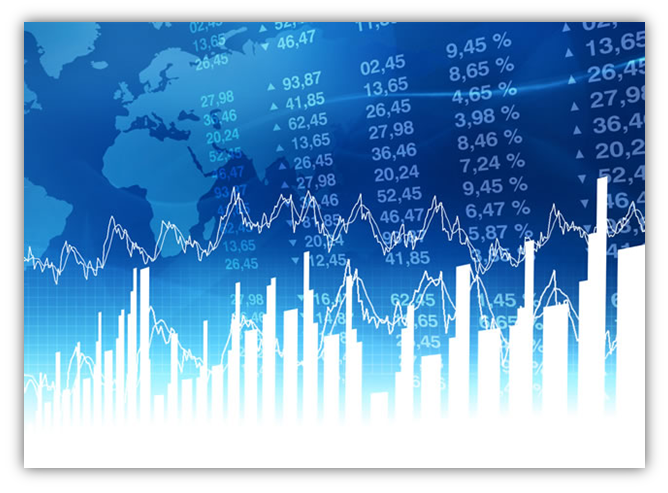
\includegraphics [width=8cm]{images/presentation3.png} \\[0.5cm]
    \begin{spacing}{1.5}
      %% \textsc{\LARGE École nationale supérieure d'informatique et de
      %%   mathématiques appliquées de Grenoble}
    \end{spacing}
  \end{flushleft}
\end{minipage}

~\vspace*{12mm}

\textsc{\Large \reportsubject}\\[0.5cm]
\HRule \\[0.4cm]
{\huge \bfseries \reporttitle}\\[0.4cm]
\HRule \\[1.5cm]

\begin{minipage}[t]{0.3\textwidth}
  \begin{flushleft} \large
    \emph{Auteurs :}\\
    \reportauthor
  \end{flushleft}
\end{minipage}
\begin{minipage}[t]{0.6\textwidth}
  \begin{flushright} \large
    \emph{Responsable :}\\Mme Estérina \textsc{Masiello} \\
    %% M.~Pierre \textsc{Bidon}
  \end{flushright}
\end{minipage}

\vfill

~\vspace*{14mm}

\begin{minipage}[t]{0.48\textwidth}
  \begin{flushleft}
    \centering 
\includegraphics [width=15mm]{images/logo-isfa.jpg} \\[0.5cm]
    \begin{spacing}{1.5}
      %% \textsc{\LARGE École nationale supérieure d'informatique et de
      %%   mathématiques appliquées de Grenoble}
    \end{spacing}
  \end{flushleft}
\end{minipage}

%~\vspace*{1mm}

{\large 17 Mai 2015}

\end{center}

\end{titlepage}

  \cleardoublepage % Dans le cas du recto verso, ajoute une page blanche si besoin
  \tableofcontents % Table des matières
  \sloppy          % Justification moins stricte : des mots ne dépasseront pas des paragraphes

\cleardoublepage  
\listoffigures  % table des figures
\cleardoublepage  
\listoftables   % table des tableaux



  %\cleardoublepage
  \section*{Introduction} % Pas de numérotation
\addcontentsline{toc}{section}{Introduction} % Ajout dans la table des matières

La théorie des copules a connu ces trois dernières décennies un essor considérable.
Ce développement a notamment vu ses applications de plus en plus nombreuses dans le domaine de la finance.
La gestion des risques, l'évaluation des rendements d'actifs, la théorie des valeurs extrêmes, requièrent des modélisations de
la dépendance et la théorie des copules permet à la finance d'accomoder la non-normalité des variables.

Avec une grande souplesse dans la mise en oeuvre de l'analyse multivariée, les copules autorisent une  sélection plus étendue des distributions conjointes des séries de données.
Les fonctions copules permettent une représentation moins naïve de la dépendance statistique fondée sur la mesure traditionnelle de corrélation qui présente des limites dans l'étude de l'interdépendance entre deux variables (cf. Embrechts et al. (1999)). 
En outre, elles autorisent des distributions de probabilités jointes moins restrictives, prenant  mieux en compte certaines caractéristiques comme l'asymétrie ou la dépendance de queue.
En somme, elles permettent de construire des distributions multidimensionnelles assez générales indépendamment des lois des marginales.

Dans ce projet, nous utiliserons cet outil puissant afin de modéliser au mieux la dépendance existant entre deux séries de données relatives 
à la vitesse maximale du vent relevées dans deux stations différentes mais proches géographiquement.

Dans une première partie, nous chercherons à décrire les données en présence et la dépendance sous-jacente au moyen de graphiques et de mesures de dépendance.
Puis, dans une seconde partie nous présenterons la copule empirique calculée sur nos données et qui nous servira de référentiel lors des tests à venir. Après un rappel théorique en début de chaque section, les parties qui suivront mettront en application différentes méthodes d'estimation sur des copules archimédiennes et des copules elliptiques :

\begin{itemize}
\item la méthode semi-paramétrique CML (Canonical Maximum Likelihood),
\item la méthode des moments,
\item les méthodes paramétriques, telles que la méthode du maximum de vraisemblance et la méthode IFM (Inference Function for Margins).
\end{itemize} 

Ensuite, nous réaliserons différents tests graphiques d'adéquation aux copules étudiées et des tests statistiques afin de retenir ou non l'adéquation des modèles de copule à nos données. 

L'ensemble des algorithmes et applications numériques ont été réalisés dans le langage de programmation $R$, dont le code est fourni avec le présent mémoire.
  
  \cleardoublepage
  
\section{Présentation des données}
%%%%%%%%%%%%%%%%%%%%%%%%%%%%%%%%%%%%%%%%%%%%%%%%%%%%%%%%%%%%%%%%%%%%%%%
\subsection{Présentation}

\subsection{Observation graphique}

\subsubsection{Scatter plot}

\subsubsection{Rank-rank plot}

\subsection{Corrélation de Pearson :  pas une mesure d’association !}

\subsection{Rho de Spearman}

\subsection{Tau de Kendall}

\section{Méthode non paramétrique d'estimation : la copule empirique}
%%%%%%%%%%%%%%%%%%%%%%%%%%%%%%%%%%%%%%%%%%%%%%%%%%%%%%%%%%%%%%%%%%%%%%%
\subsection{Choix d'une copule théorique}


\section{Méthode paramétriques d'estimation}
%%%%%%%%%%%%%%%%%%%%%%%%%%%%%%%%%%%%%%%%%%%%%%%%%%%%%%%%%%%%%%%%%%%%%%%

\subsection{Méthode du maximum de vraisemblance}

\subsection{Méthode IFM (Inference Function for Margins)}


\section{Méthode semi-paramétrique d'estimation (CML)}
%%%%%%%%%%%%%%%%%%%%%%%%%%%%%%%%%%%%%%%%%%%%%%%%%%%%%%%%%%%%%%%%%%%%%%%

Dans cette section, nous allons utiliser la méthode CML (méthode semi-paramétrique) afin d'estimer le paramètre des différentes copules retenues pour modéliser la dépendance entre les données sur Saint-Martin et celles sur Echirolles.

\subsection{Copule de Clayton}

\subsection{Copule de Gumbel}

\subsection{Copule de Franck}

\subsection{Copule normale}

\subsection{Copule de Student}

\section{Méthode des moments : inversion du tau de Kendall}
%%%%%%%%%%%%%%%%%%%%%%%%%%%%%%%%%%%%%%%%%%%%%%%%%%%%%%%%%%%%%%%%%%%%%%%

Dans cette partie, nous utiliserons la méthode des moments pour estimer le paramètre des copules retenues afin de modéliser la dépendance entre les données sur Saint-Martin et celles sur Echirolles.

\subsection{Copule de Clayton}

\subsection{Copule de Gumbel}

\subsection{Copule de Franck}

\subsection{Copule normale}

\subsection{Copule de Student}

\section{Test graphique d'adéquation à la copule : le Kendall plot}
%%%%%%%%%%%%%%%%%%%%%%%%%%%%%%%%%%%%%%%%%%%%%%%%%%%%%%%%%%%%%%%%%%%%%%%

\subsection{Dépendogramme empirique et dépendogramme théorique}

\subsection{K-plot}

\section{Test statistique d'adéquation à la copule : le Kendall plot}
%%%%%%%%%%%%%%%%%%%%%%%%%%%%%%%%%%%%%%%%%%%%%%%%%%%%%%%%%%%%%%%%%%%%%%%

\subsection{Test de Kolmogorov-Smirnov}

\subsection{La statistique de Cramér-von Mises}

\subsection{Estimation du seuil critique par bootstrap paramétrique}





TODO   TODO   TODO   TODO



%% \noindent%
%% \begin{figure}[H]
%%     \begin{center}
%%       \includegraphics[width=17 cm, angle=0]{./pictures/logchrono1.png}
%%       \centering\caption{\label{2}Logarithme du total des importations de gaz naturel}
%%     \end{center}
%% \end{figure}




  \cleardoublepage
  %\include{latex_files/partie2}
  % \cleardoublepage
  %\include{latex_files/partie3}
  % \cleardoublepage
  %\include{latex_files/partie4}
   %\cleardoublepage
  \section*{Conclusion}
\addcontentsline{toc}{section}{Conclusion}

Lors de ce projet, nous avons pu mettre en application la théorie des copules. Cette théorie voit tout son intérêt dans la gestion des risques et plus généralement dans le domaine de l'actuariat et de la finance. Grâce à ce puissant outil statistique, nous avons cherché à proposer une modélisation de la dépendance entre les valeurs de la vitesse maximale du vent enregistrées par deux stations distinctes. Les procédures d'estimation des copules ont été réalisées selon diverses méthodes (paramétriques, semi-paramétriques et non-paramétriques) afin d'estimer au mieux les paramètres de chaque copule (et les paramètres des lois marginales). Ensuite, nous avons retenu la moyenne des paramètres obtenu par ces différentes méthodes pour réaliser un ensemble de tests graphiques et de tests statistiques afin de comparer l'adéquation des modèles de copules étudiés à nos données. Ainsi, il ressort de cette étude que la copule normale permet de représenter au mieux la dépendance positive existant entre les valeurs des deux stations.





\clearpage

\clearpage
%% ANNEXE
\appendix
%\section{Annexe}
%\label{refCode}
\begin{lstlisting}[language=cli, name=Sim, caption=Code R]


\end{lstlisting}


\cleardoublepage
   \phantomsection\addcontentsline{toc}{section}{Références}
\begin{thebibliography}{ABC}	
%%    \bibitem[REF]{reference} auteur. \emph{titre}. édition, année.
%%    \bibitem[LPP]{lpp} Rolland. \emph{LaTeX par la
%%    pratique}. O'Reilly, 1999.


\bibitem{reference}\label{ref1} C. Robert, \emph{Séries temporelles}, ISFA, support de cours, 2014.


\end{thebibliography}

%% \textbf{Sources des données financières sur l'inflation} :

%% \url{www.inflation.eu}


%% \include{latex_files/partie5}
%%    \cleardoublepage
%%%%%%%%%%%%%%%%% FIN DU DOCUMENT %%%%%%%%%%%%%%%%%%%%%%

\end{document}


